\section{Discussion}\label{sec:discussion}

\subsection{Potential issues}

\subsubsection{The same symbols can represent different concepts.}

Upon inspecting low-dimensional state cloud projections, we observed the presence of distinctive clusters across latent space (see Fig. \ref{fig:plant}). For instance, the state cloud of the symbol "plant" appears to be populated by at least three clusters. To investigate this, we ran a K-means clustering ($K=3$) procedure on the "plant" state cloud and surfaced the contexts which yielded contextual embeddings closest to the cluster centroids. Upon inspection of those contexts, we noticed that the context sets contained distinctive word senses, roughly corresponding to (1) plant objects, (2) the action of planting, and (3) factories (see Table \ref{tab:samples}).

\begin{figure}[h]
    \centering
    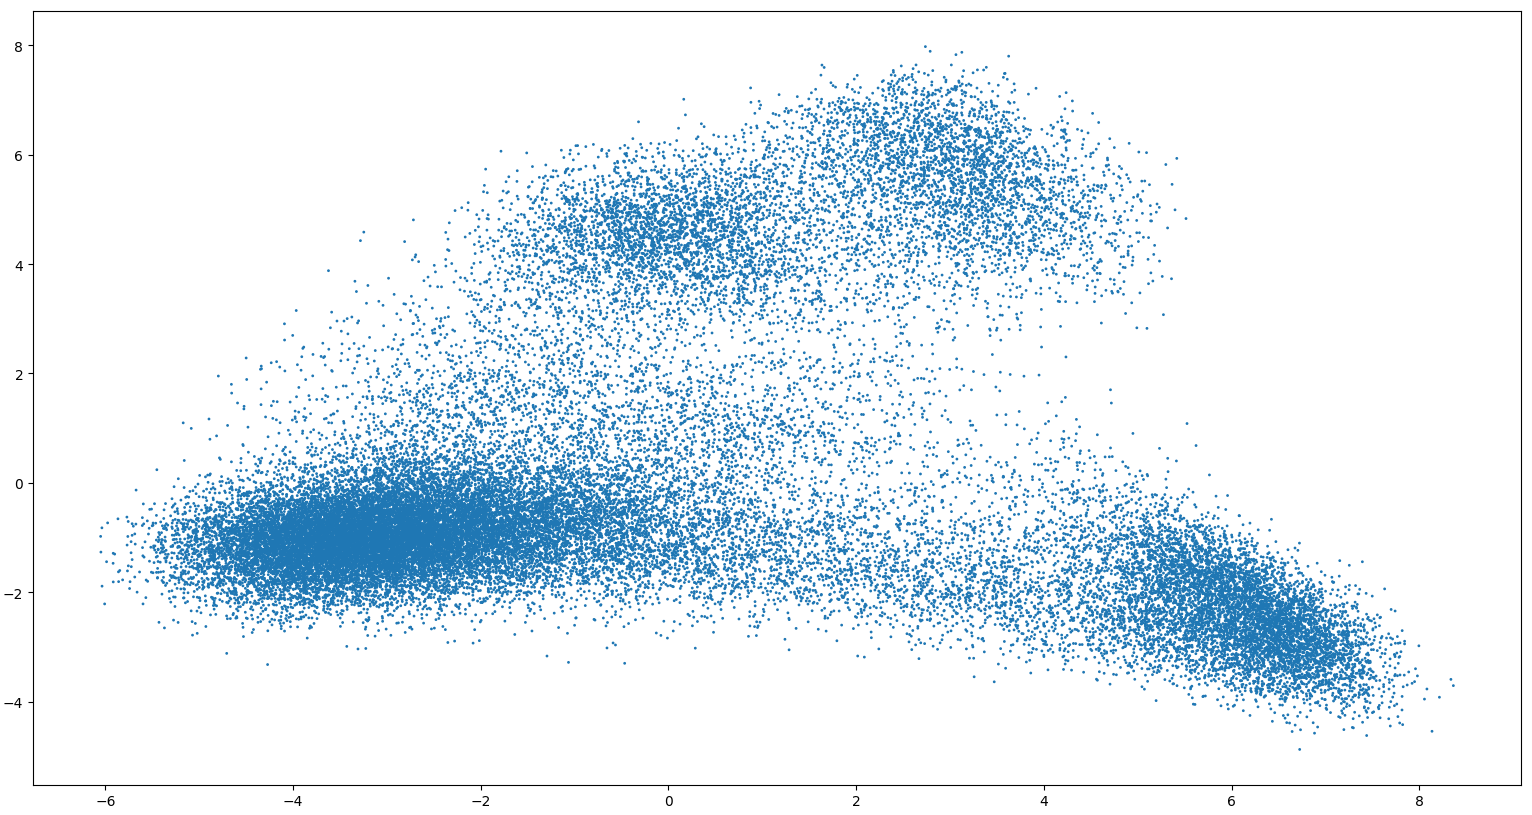
\includegraphics[width=0.45\textwidth]{img/plant.png}
    \caption{2D PCA projection of the state cloud associated with the symbol "plant"}\label{fig:plant}
\end{figure}

\begin{table}[!bp]
    \caption{Context samples by K-means cluster of "plant" state cloud.}
    \label{tab:samples}
    \begin{tabular}{|l|l|}
        \hline
        \textbf{Cluster} & \textbf{Sample context} \\
        \hline
        1 & \parbox{0.7\linewidth}{absently, i raised the blinds so that the plant was able to soak in the
        impromptu sunshine.} \\
        \hline
        & \parbox{0.7\linewidth}{i’ve brought you over a few macramé plant hangers to decorate your room.} \\
        \hline
        2 & \parbox{0.7\linewidth}{i wanted to plant them myself.} \\
        \hline
         & \parbox{0.7\linewidth}{she’ll just plant new ones and start all over again.} \\
        \hline
        3 & \parbox{0.7\linewidth}{the computers running the plant were all infected, of course.} \\
        \hline
        & \parbox{0.7\linewidth}{it was plant shutdown for two weeks.} \\
        \hline
    \end{tabular}
\end{table}

This diversity of meanings assumed by the same symbol across the text corpus casts doubt on our assumption of there being a one-to-one correspondence between symbols and graph nodes. An intermediate clustering step might be effective in decoupling different word senses and producing different state clouds, though the issue of how many senses are there per symbol is non-trivial. Similar to how words themselves appear to discretely quantize the otherwise continuous semantic space, finite word senses as "subsymbols" run into similar trade-offs between sparsity and accuracy.

\subsubsection{State clouds are non-linear.}

While we employ conceptors as compact elliptical objects which approximate high-dimensional state clouds of contextual embeddings, their limited expressivity might fail to capture the intricate non-linear layout of real-world embeddings. Low-dimensional PCA projections of several state clouds of BERT embeddings radically diverge from Gaussian distributions, bringing into question the suitability of elliptical conceptors to represent them (see Fig. \ref{fig:earth}). However, we note that state clouds of less ambiguous terms (i.e. limited number of word senses) appear more well-formed. Non-linearities might arise mainly from diverse word senses being assumed by the same symbols.

\begin{figure}[h]
    \centering
    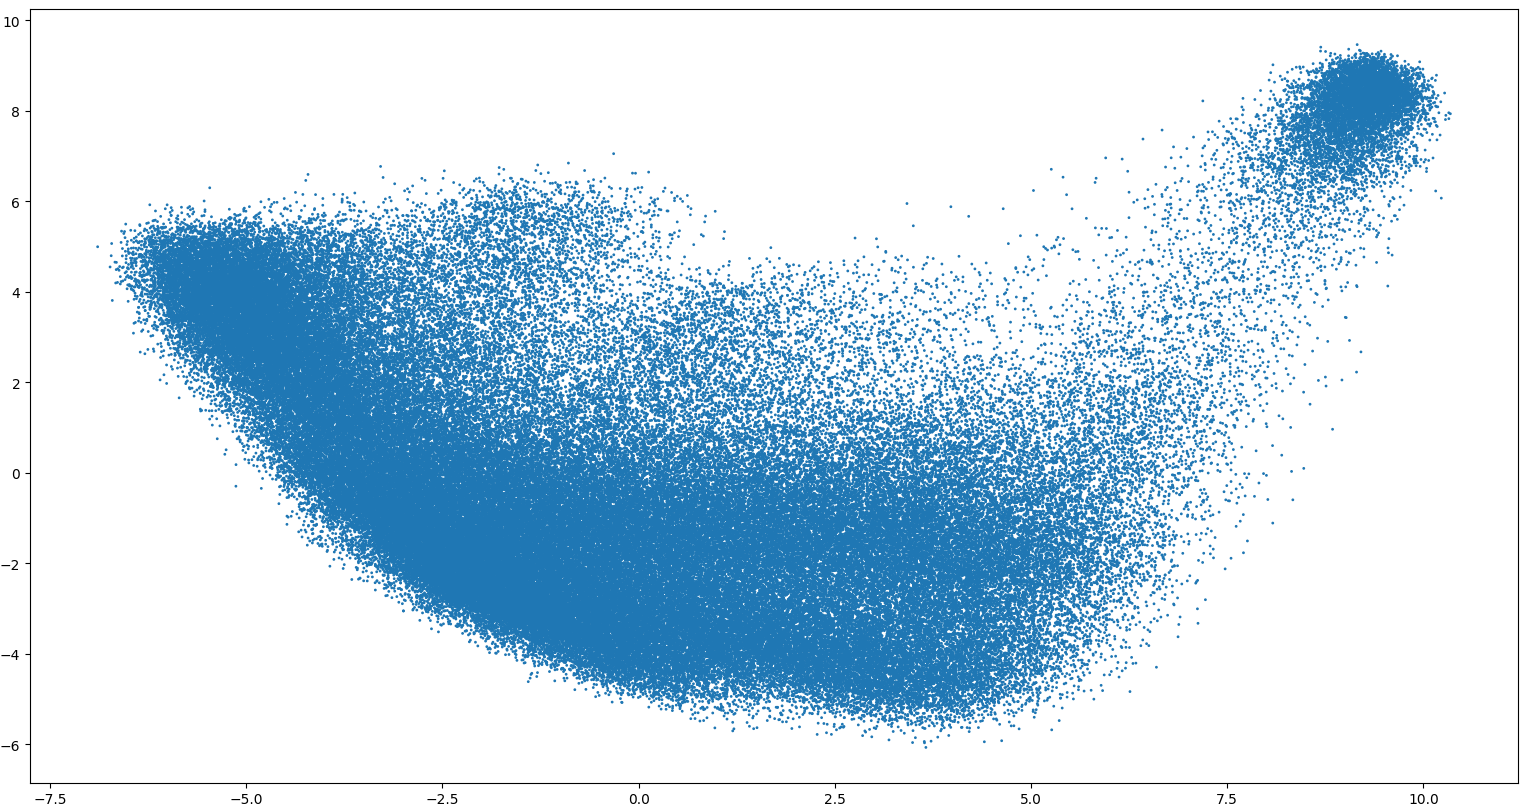
\includegraphics[width=0.45\textwidth]{img/earth.png}
    \caption{2D PCA projection of the state cloud associated with the symbol "earth"}\label{fig:earth}
\end{figure}

\subsubsection{NSC requires many exemplars.}

The central role of state clouds in NSC means that the technique is highly dependent on a large number of occurences and contexts for each concept analyzed. This makes it difficult to interpret the model's internal representations with respect to obscure tokens, as those are extremely rare in natural datasets. However, synthetic datasets might address this issue, provided the ability to synthesize a wide range of unique contexts for an arbitrary concept.

\subsubsection{NSC is influenced by the choice of auxiliary data.}

\textbf{NSC does not only require the model under investigation in order to work. There is also the requirement of an auxiliary dataset which contains a wide range of exemplars in different contexts. NSC then uses those exemplars in order to approximate the overarching state cloud with a conceptor object. However, the particular choice of dataset in which the concept instances are to be found has a high influence on the output knowledge graph.}

\textbf{For instance, consider two senses of the symbol "property." It might refer to (1) a characteristic, or (2) a real estate asset, among other senses. Different datasets might contain quantitatively distinct distributions of the meaning of "property" across latent space. One predominantly containing text about real estate matters might be skewed towards considering sense (2) above as the most pervasive one. In contrast, a dataset containing text about the physical properties of certain materials might be skewed in the other direction, towards considering sense (1) above as the most typical one.}

\textbf{One might be tempted to simply aim for large datasets in order to alleviate this concern. Unfortunately, the issue as hand is not that certain senses are not represented enough through exemplars in order for their meaning to be captured. Rather, it is specifically an issue of representativity in the resulting population of meanings. This has two implications, one concerning industry applications, and one concerning epistemics. The first is that, in practice, one would have to identify an auxiliary dataset which is representative enough of the concepts desired to be placed in the resulting knowledge graph. For instance, if one aims to investigate an ML model's internalized representations related to real estate matters, one concerning material science would be a poor choice of auxiliary dataset. The second implication hints at the fact that transparency tools like the ones used broadly in XAI can only meaningfully relate latent representations to the world models of people who authored the datasets. If one was to apply NSC on a book corpus, as we did, it would be unlikely for terms like "entity," "object", or "thing" to be organized in an ontology in the same way a logician might organize them.}

\subsubsection{NSC output graph is heavily influenced by the graph search objective.}

The graph search process employed to output a knowledge graph is highly sensitive to the search objective. Reaching a balance between the functional-grounded terms (e.g. faithfulness to detected abstraction ordering) and human-grounded terms (e.g. sparsity) is difficult to achieve manually. Often, one component of the linear combination tends dominates the others (see Fig. \ref{fig:children} and Fig. \ref{fig:pruning}). This balance is especially difficult to find with higher number of concepts, bringing the scalability of NSC into question. However, normalizing the objective's components based on the number of concepts being analyzed greatly improved robustness.

\begin{figure}[h]
\centering
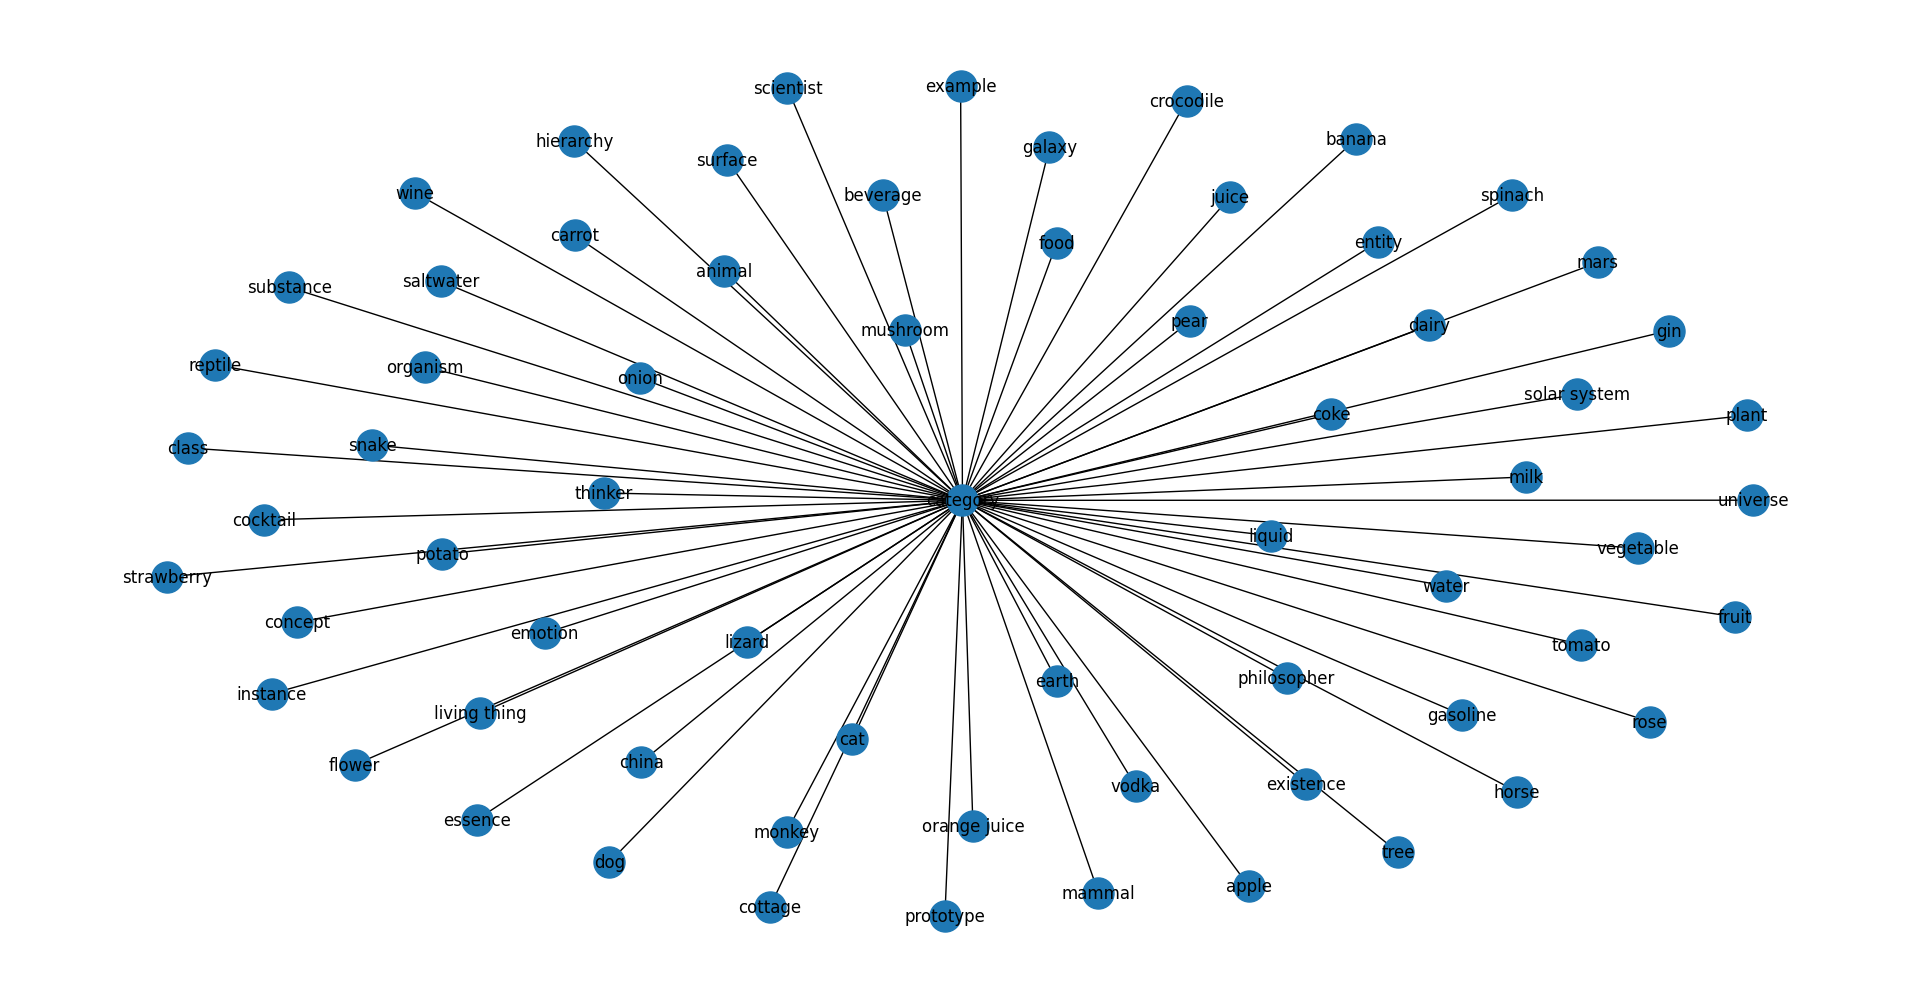
\includegraphics[width=0.45\textwidth]{img/too_much_pruning.png}
\caption{NSC output graph after undervaluing children count per node constraints.}\label{fig:children}
\end{figure}

\begin{figure}[h]
\centering
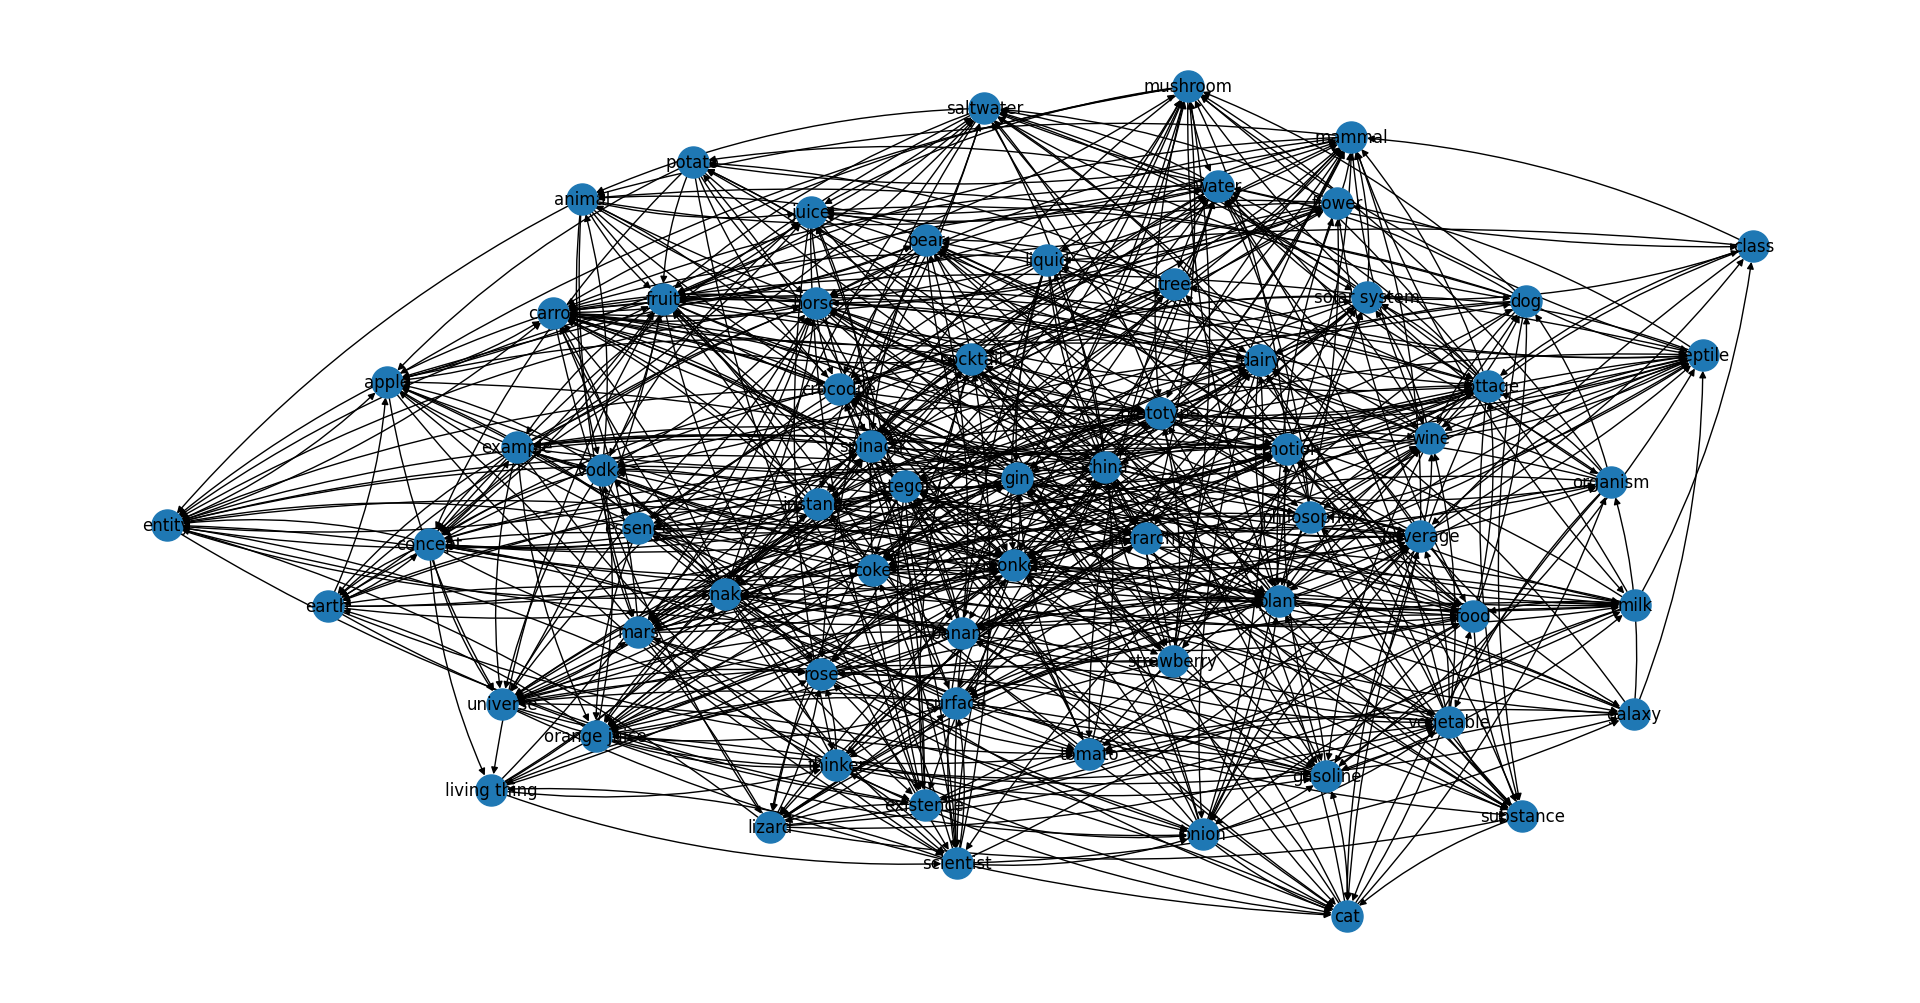
\includegraphics[width=0.45\textwidth]{img/short_run.png}
\caption{NSC output graph after undervaluing arc pruning.}\label{fig:pruning}
\end{figure}

\subsection{Future work}

\subsubsection{Beyond linear conceptors}

Non-linear variations of classical conceptors might be used to capture the internal structure of high-dimensional state clouds of contextual embeddings better than the original elliptical objects. It had been suggested that shallow MLPs could be employed for this task, yet this brings additional questions of interpretability. As we attempt to model high-dimensional representations ever more accurately, we might be forced to depart from sparse human-grounded explanations, an issue resembling the adequacy-fluency trade-off in machine translation.

\textbf{However, an issue arises when addressing the spatial intuition and theoretical grounding of the abstraction ordering of two conceptors. While this notion is well-defined for linear conceptors (i.e. the ones employed in this work), it is currently an ambiguous notion when it comes to non-linear conceptors. In linear conceptors, abstraction ordering reduces to an evaluation of whether the difference matrix between two conceptors is positive definite. In practice, due to the high amount of noise involved in non-synthetic datasets, we resort to merely approximating this property, by using heuristics based on the eigenvalues of the difference matrix. In non-linear conceptors potentially making use of non-trivial neural networks, the expression of abstraction ordering also becomes non-trivial -- the subject of future work.} 

\subsubsection{Beyond abstraction ordering}

While this work focuses solely on the meronymous IS\_A relationship of abstraction between to concepts, it's conceivable that the difference matrix computed in NSC as an intermediate step contains a rich representation of other relationships between concepts. This is reminiscent of the seemingly algebraic properties of prototype word embeddings (e.g. "king" + "woman" - "man" ~ "queen"), which appear to encode diverse analogies and conceptual relationships. The relative spatial layout of entire state clouds might provide similar information.

\textbf{However, mathematical objects depicting the aggregate shape of high-dimensional space clouds are likely to capture more information about the semantics of the symbols involved, compared to more rudimentary single prototype embeddings. Assuming the benefit of employing more expressive representation which stays faithful to large sets of exemplars at once, the difference matrices obtained from pairs of conceptor objects might also represent more nuance compared to the less expressive vector of displacement between prototype embeddings.} 

\subsubsection{Beyond token embeddings}

\textbf{The present work focuses solely on extracting a part-whole knowledge graph from the state clouds comprised of contextual embeddings of text tokens (e.g. "juice") or short sequences of such tokens (e.g. "orange juice"). In section 1, however, we mention that NSC is modality-agnostic, in that it can theoretically be employed to distill knowledge graphs from embeddings of other modalities. One possible way of accomplishing that is by pooling together the data points associated with a certain class in an image classification setting. The class would then be identified with a concept based on its label (e.g. "fruit"), while its associated state cloud would not consist in a set of contextual embeddings, as in the case of text, but would be composed of a set of image embeddings generated for entire images (e.g. thousands of images of fruits). By learning conceptors from those state clouds, relating them using abstraction ordering heuristics, and searching for an appropriate knowledge graph structure, it is likely that meaningful meronymous structures would arise. Similar approaches could be employed for yet other modalities. For instance, audio classification datasets would give way to ontologies of audio concepts. Alternatively, datasets comprising video or 3D point clouds, together with labels unifying them in meaningful classes, might also lead to XAI tools in those other modalities.}

\subsubsection{Alternative abstraction heuristics}

\textbf{In the present work, we employ a rather specific heuristic for quantifying the relation of abstraction between two conceptors. For completeness, we mean-pool the eigenvalues of their difference matrix. Large positive values indicate the first conceptor is deemed to be more abstract than the second, while large negative values indicate the reverse. Values close to zero indicate a limited relation of abstraction between the two.}

\textbf{However, there might be other -- better mathematically-motivated -- ways of quantifying this relation. For instance, one might opt for different pooling mechanisms (e.g. median), which are more robust against outliers. Alternatively, one might eliminate the eigenvalue pooling mechanism entirely, and focus instead on the \textit{ratio} between positive and negative eigenvalues.}